%=======================================================================
\section{AMR Component} \label{s:component-amr}
%=======================================================================

The \code{Mesh} component defines the data structures and associated
parameters for the ``inter-resolution'' aspect of data fields on
distributed AMR hierarchies.  The ``intra-resolution'' aspects are
defined using the closely related \code{Array} component.  Both
patch-based AMR, ala \enzo, and octree-like-based AMR datastructures
are supported.  Support for associating \code{Particle} groups with
\code{Array}'s in an AMR hierarchy is also included in the
\code{Mesh} component.

Tentative features of \code{Mesh} support in Cello include the following: 

\begin{itemize}
%
    \item Octree-like AMR. We want to eliminate the need for heuristic
      grid placement algorithms and neighbor searches, to simplify
      load balancing, eliminate the need for persistent ghost zones,
      and to improve the scalability of representing the
      data-structure in a distributed memory. (Caveat: ``Wish'' W010
      by Norman is to include structured AMR capability).
%
    \item Full unilevel efficiency. A single-level AMR ``hierarchy''
      should reduce to a single \code{Array}. This is different from Enzo,
      which allocates O(P) grid patches per MPI-process, and involves
      costly and unnecessary neighbor searches.
%
    \item Partitioned ``inter-resolution'' and ``intra-resolution''
      management. The \code{Mesh} component defines and manages the
      inter-refinement structure, whereas the \code{Array} component
      defines and manages the intra-resolution structures.
%
    \item Flexibility between levels. Supports refinement-by-two
      (octree), refinement-by-four (64-tree), refinement-by-7
      (343-tree), etc. Also perhaps ``in-between'' ( e.g. ($2 \times 4
      \times 4$)-tree ) with corresponding rectangular
      arrays. Restricting to, e.g., only $4^3$ grid patches could be
      helpful for highly-tuned numerical methods, cache sizes, or to
      maintain uniform parallel task sizes.
%
    \item Flexibility within levels. Flexibility in array sizes, for
      example, $4^3$, $7^3$, etc., to match flexibility of AMR tree
      shapes, and allow refinement by \code{Array} arrays instead of
      by \code{Mesh} tree structure.
%
    \item ``Smooth'' refinement. Intermediate ``pseudo-levels'',
      implemented by introducing a ``bridge of \code{Array}'s, can be
      introduced between existing hierarchy levels to maintain smooth
      resolution transitions. This should enable using high refinement
      ratios (e.g. $16^3$-trees) for more efficient targeting of
      features, but without introducing undue grid resolution effects.
%
    \item Optimized \code{Mesh} - \code{Array} data-structure
      partitioning. Efficiency can be improved by optimizing
      \code{Array}s versus the \code{Mesh} refinement tree. For
      example, if a domain is flagged to be refined everywhere, then
      the \code{Mesh} data-structure detects this and collapses back to
      a single but larger \code{Array}.
%
    \item Scalable depth. We want to allow ``massively deep''
      AMR hierarchies without limits based on floating point
      precision or limited integer range.  For example, positions of
      particles associated with a \code{Mesh} \code{Patch} are stored
      with particle positions normalized between $-1.0 < x < 1.0$ to
      enable more than sufficient precision, even with single precision.
\end{itemize}

\subsection{Design issues}

\begin{itemize}
    \item How to decide tradeoffs between \code{Array} resolution and \code{Mesh}
      refinement?
    \item What support is needed for Particles?
    \item How to handle remeshing?
    \item How to dynamically adjust tree size (23,43, 83,
      etc.)(adaptive adaptivity)
    \item How to deal with ghost zones
    \item What operations needed for load balancing
\end{itemize}

\subsection{\code{Mesh} supporting classes}

\begin{itemize}
    \item \code{Mesh}
    \begin{itemize}
          \item \code{Array}
          \item \code{Particles}
          \item \code{Patch}
          \item \code{Box}: 
    \end{itemize}
\end{itemize}

\code{Mesh} operations

\code{Mesh} class hierarchy

Operations

The \code{\code{Mesh}} component accesses the \code{Array} component to
define the ``intra-resolution'' aspect of field data on an AMR
hierarchy, and the \code{Particles} component to define particles on
the AMR hierarchy.  

to, such as number of mesh levels, grid patch properties,
rebuild algorithm, dynamic load balancing, refinement criteria, etc.

Hierarchy
\code{Array}


\begin{itemize}
\item hierarchy
\begin{item}
\item min\_levels 
\item max\_levels 
\end{item}
\item level
\item grid
\begin{itemize}
\item min\_size
\item max\_size
\item max\_aspect
\item quantum
\end{itemize}
\end{itemize}

\centerline{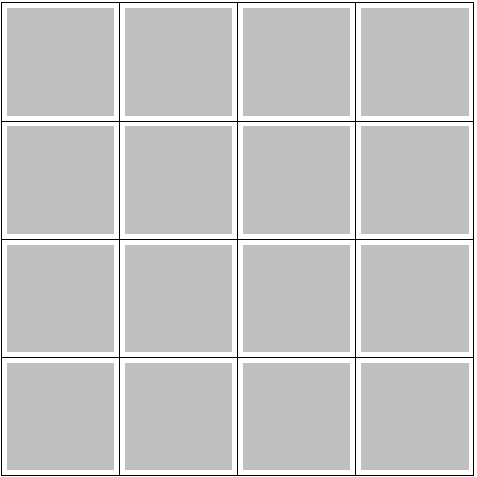
\includegraphics[width=1.8in]{amr4-1.pdf} \ \
            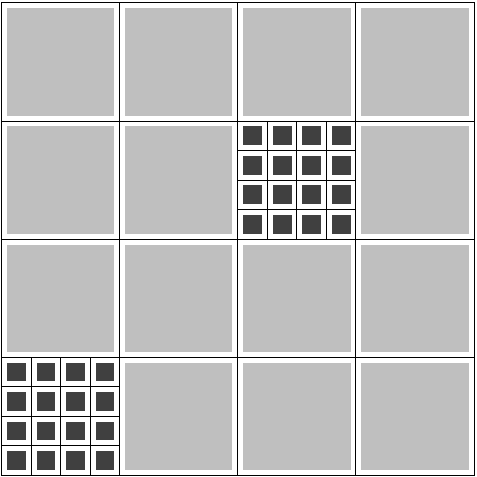
\includegraphics[width=1.8in]{amr4-2.pdf} \ \
            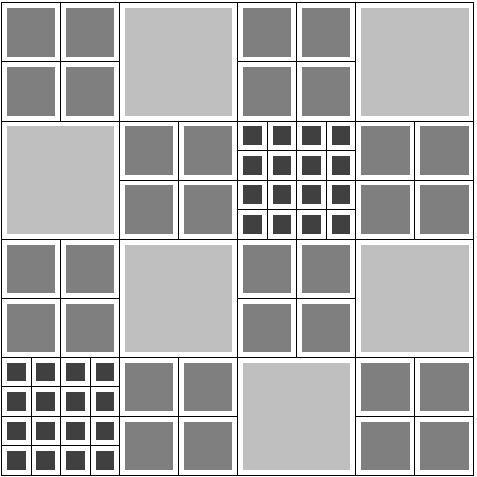
\includegraphics[width=1.8in]{amr4-3.pdf}}

\centerline{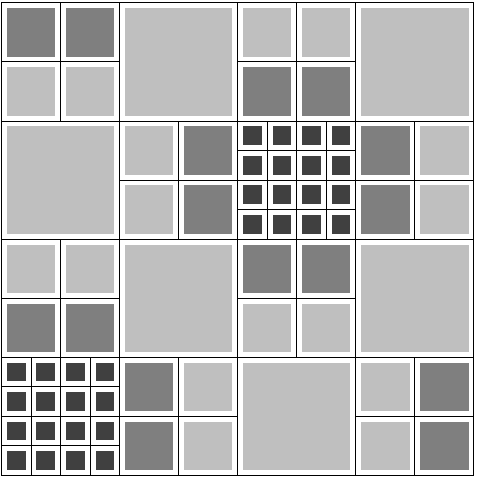
\includegraphics[width=1.8in]{amr4-4.pdf} \ \
            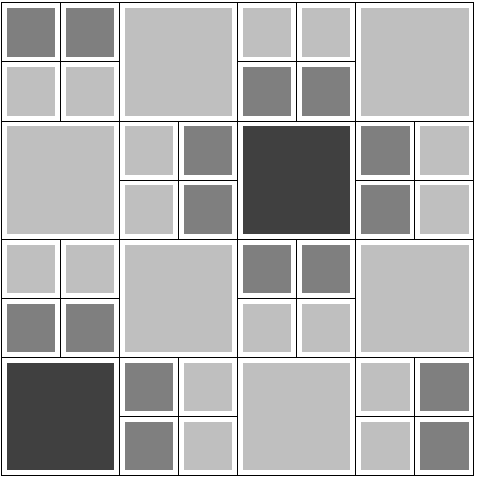
\includegraphics[width=1.8in]{amr4-5.pdf} \ \
            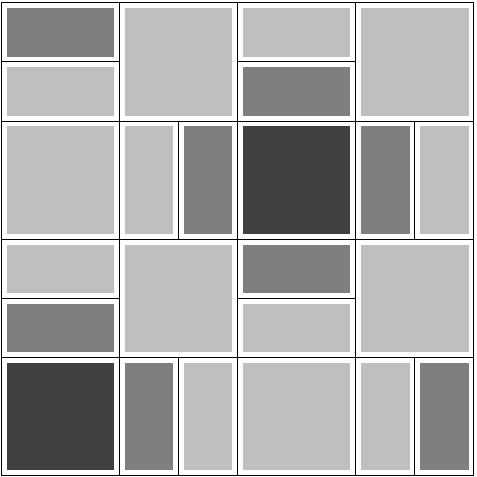
\includegraphics[width=1.8in]{amr4-6.pdf}}
\centerline{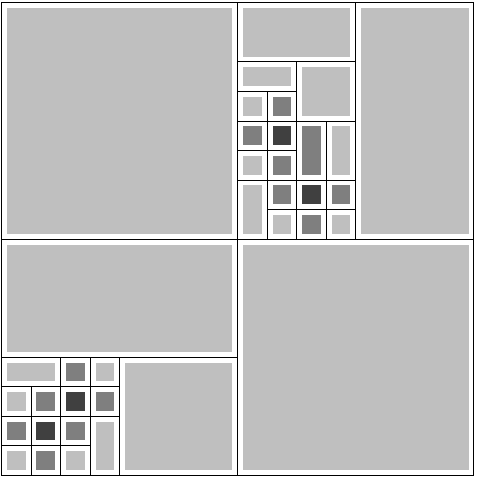
\includegraphics[width=1.8in]{amr4-7.pdf}}

% \centerline{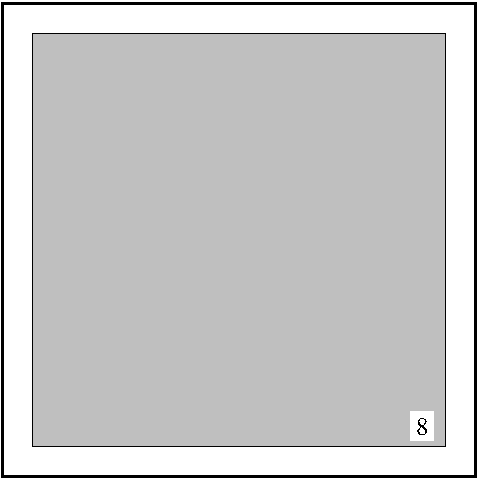
\includegraphics[width=1.8in]{amr2-1.pdf} \ \
%             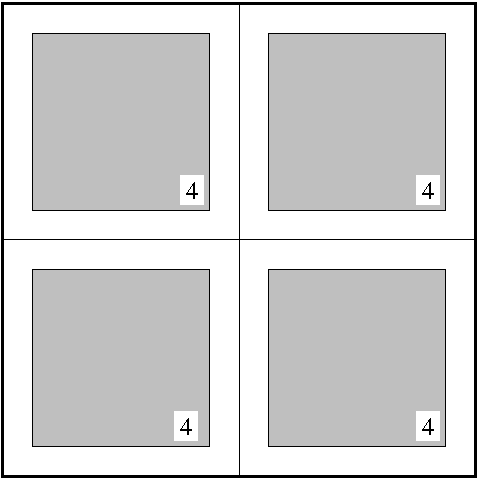
\includegraphics[width=1.8in]{amr2-2.pdf} \ \
%             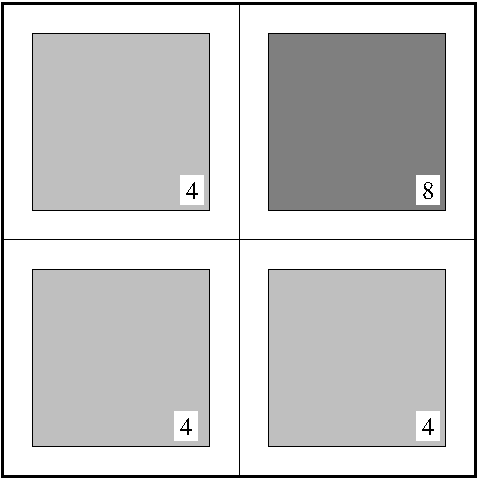
\includegraphics[width=1.8in]{amr2-3.pdf}}
% \ \\
% \centerline{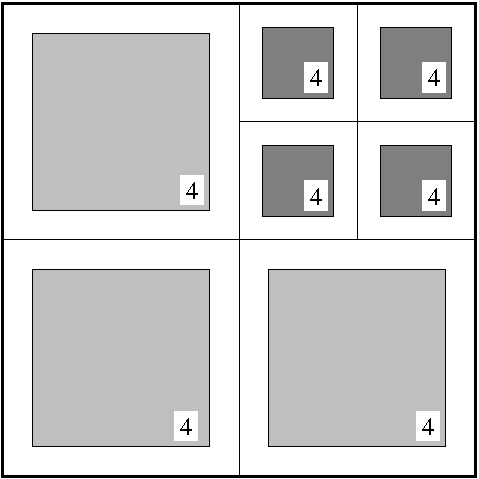
\includegraphics[width=1.8in]{amr2-4.pdf} \ \
%             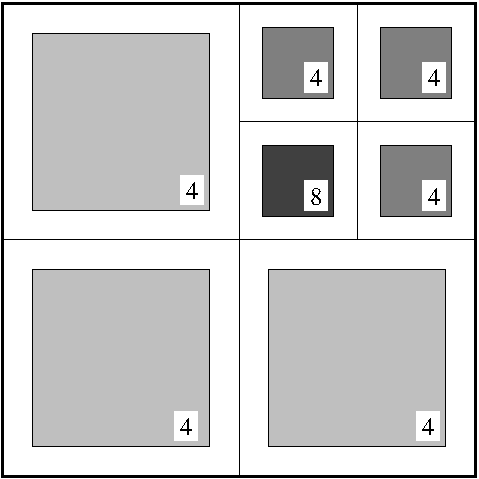
\includegraphics[width=1.8in]{amr2-5.pdf} \ \
%             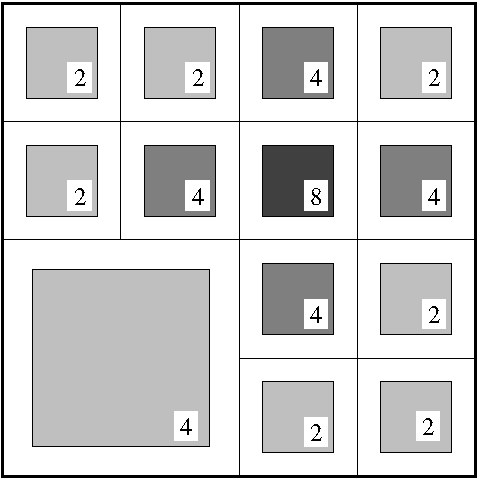
\includegraphics[width=1.8in]{amr2-7.pdf}}
% \ \\
% \centerline{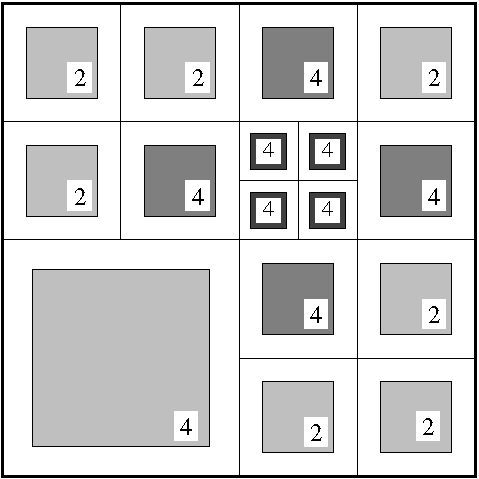
\includegraphics[width=1.8in]{amr2-8.pdf} \ \
%             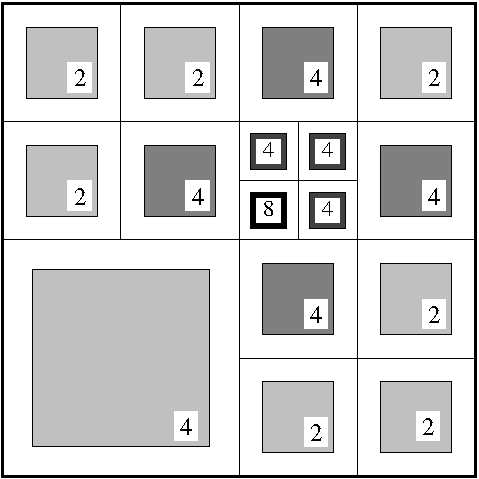
\includegraphics[width=1.8in]{amr2-9.pdf} \ \
%             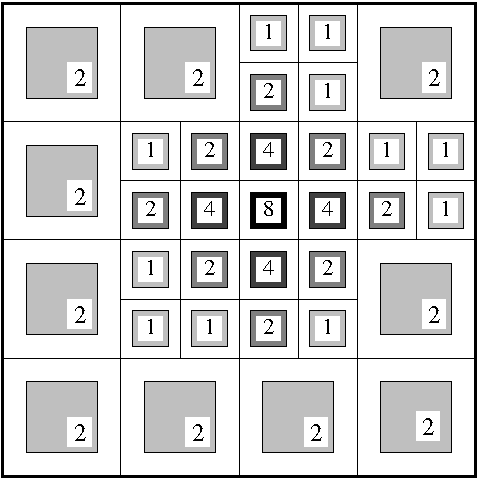
\includegraphics[width=1.8in]{amr2-11.pdf}}

%-----------------------------------------------------------------------
\subsection{Use Cases}
%-----------------------------------------------------------------------
%-----------------------------------------------------------------------
\subsection{Parameters}
%-----------------------------------------------------------------------
